% Hlavicka pro protokoly z fyzikalniho praktika.
% Verze pro: LaTeX
% Verze hlavicky: 22. 2. 2007
% Autor: Ustav fyziky kondenzovanych latek
% Ke stazeni: www.physics.muni.cz/ufkl/Vyuka/
% Licence: volne k pouziti, nejlepe k vcasnemu odevzdani protokolu z Vaseho mereni.

\documentclass[a4paper,11pt]{article}

% Kodovani (cestiny) v dokumentu: utf-8
%\usepackage[cp1250]{inputenc}	% Omezena stredoevropska kodova stranka, pouze MSW.
\usepackage[utf8]{inputenc}	% Doporucujeme pouzivat UTF-8 (unicode).
\usepackage[T1]{fontenc}
\usepackage{lmodern}

%%% Nemente:
\usepackage[margin=2cm]{geometry}
\newtoks\jmenopraktika \newtoks\jmeno \newtoks\datum
\newtoks\obor \newtoks\skupina \newtoks\rocnik \newtoks\semestr
\newtoks\cisloulohy \newtoks\jmenoulohy
\newtoks\tlak \newtoks\teplota \newtoks\vlhkost
\usepackage{amsmath}
\usepackage{mathtools}
\usepackage{graphicx}
\usepackage{multirow}

\usepackage{pgfplotstable} 
\usepackage{booktabs}

\graphicspath{ {./images/} }
%%% Nemente - konec.


%%%%%%%%%%% Doplnte pozadovane polozky:

\jmenopraktika={Fyzikální praktikum 3}  % nahradte jmenem vaseho predmetu
\jmeno={Artem Gorodilov}            % nahradte jmenem mericiho
\datum={8. ~dubna  2024}        % nahradte datem mereni ulohy
\obor={Astrofyzika}                     % nahradte zkratkou vami studovaneho oboru
\skupina={Po 14:00}            % nahradte dobou vyuky vasi seminarni skupiny
\rocnik={II}                  % nahradte rocnikem, ve kterem studujete
\semestr={II}                 % nahradte semestrem, ve kterem studujete

\cisloulohy={J}               % nahradte cislem merene ulohy
\jmenoulohy={Operační zesilovač} % nahradte jmenem merene ulohy

\tlak={979}                   % nahradte tlakem pri mereni (v hPa)
\teplota={21.4}               % nahradte teplotou pri mereni (ve stupnich Celsia)
\vlhkost={46}               % nahradte vlhkosti vzduchu pri mereni (v %)

%%%%%%%%%%% Konec pozadovanych polozek.


%%%%%%%%%%% Uzitecne balicky:
\usepackage[czech]{babel}
\usepackage{graphicx}
\usepackage{amsmath}
\usepackage{xspace}
\usepackage{url}
\usepackage{indentfirst}
\usepackage{listings}
\usepackage{subcaption}
\usepackage{caption}
\usepackage{tabularx}
\usepackage[labelformat=parens,labelsep=quad,skip=3pt]{caption}

%%%%%% Zamezeni parchantu:
\widowpenalty 10000 \clubpenalty 10000 \displaywidowpenalty 10000
%%%%%% Parametry pro moznost vsazeni vetsiho poctu obrazku na stranku
\setcounter{topnumber}{3}	  % max. pocet floatu nahore (specifikace t)
\setcounter{bottomnumber}{3}	  % max. pocet floatu dole (specifikace b)
\setcounter{totalnumber}{6}	  % max. pocet floatu na strance celkem
\renewcommand\topfraction{0.9}	  % max podil stranky pro floaty nahore
\renewcommand\bottomfraction{0.9} % max podil stranky pro floaty dole
\renewcommand\textfraction{0.1}	  % min podil stranky, ktery musi obsahovat text
\intextsep=8mm \textfloatsep=8mm  %\intextsep pro ulozeni [h] floatu a \textfloatsep pro [b] or [t]

% Tecky za cisly sekci:
\renewcommand{\thesection}{\arabic{section}.}
\renewcommand{\thesubsection}{\thesection\arabic{subsection}.}
% Jednopismenna mezera mezi cislem a nazvem kapitoly:
\makeatletter \def\@seccntformat#1{\csname the#1\endcsname\hspace{1ex}} \makeatother

\begin{document}

\thispagestyle{empty}

{
\begin{center}
\sf 
{\Large Ústav fyzikální elektroniky PřF MU} \\
\bigskip
{\huge \bfseries FYZIKÁLNÍ PRAKTIKUM} \\
\bigskip
{\Large \the\jmenopraktika}
\end{center}

\bigskip

\sf
\noindent
\setlength{\arrayrulewidth}{1pt}
\begin{tabular*}{\textwidth}{@{\extracolsep{\fill}} l l}
\large {\bfseries Zpracoval:}  \the\jmeno & \large  {\bfseries Naměřeno:} \the\datum\\[2mm]
\large  {\bfseries Obor:} \the\obor  \hspace{40mm}  {\bfseries Skupina:} \the\skupina %
%{\bfseries Ročník:} \the\rocnik \hspace{5mm} {\bfseries Semestr:} \the\semestr  
&\large {\bfseries Testováno:}\\
\\
\hline
\end{tabular*}
}

\bigskip

{
\sf
\noindent \begin{tabular}{p{3cm} p{0.6\textwidth}}
\Large  Úloha č. {\bfseries \the\cisloulohy:} \par
\smallskip
% $T=\the\teplota$~$^\circ$C \par
% $p=\the\tlak$~hPa \par
% $\varphi=\the\vlhkost$~\%
&\Large \bfseries \the\jmenoulohy  \\[2mm]
\end{tabular}
}

\vskip10pt
    \begin{minipage}[t]{0.5\textwidth} 
        \section{Zadání}    
            \begin{enumerate}
                \item Určit, jak komparátor reaguje na různá vstupní napětí a jejich rozdíly. 
                \item Ověřit platnost vzorce (1) pro invertující zesilovač.
                \par Určit šířku pásma daného zapojení operačního zesilovače.
                \item Změřit závislost zesílení na frekvenci a z grafu této závislosti určit šířku pásma dolnofrekvenčního zesilovače.
                \item Ověřit platnost vzorce (3) pro neinvertující zesilovač.
                \item Ověřit platnost vzorce (4) pro rozdílový zesilovač.
                \item Zjistit, který ze zesilovačů znázorněných na obrázku (7) plní funkci derivačního zesilovače. 
            \end{enumerate}
        \section{Teorie}
            \subsection{Operační zesilovač}
                Operační zesilovač je běžně používaný elektronický prvek. Jeho hlavní funkcí je zesílení rozdílu napětí mezi vstupy, čímž dokáže vyprodukovat napětí mnohonásobně vyšší než je tento rozdíl. Skutečné operační zesilovače mohou poskytovat zesílení od míň než 1000 až po více než milion. Frekvenční rozsah operačních zesilovačů se pohybuje od několika kHz do stovek MHz. Při vyšších frekvencích dochází ke snížení zesílení a k fázovému posunu mezi vstupem a výstupem, což je důležité pro systémy s vysokou frekvencí a zpětnovazební obvody, kde by zpoždění mohlo vést k nestabilitě systému.
    \end{minipage}
    \hspace{10pt}
    \begin{minipage}[t]{0.5\textwidth} 
                Schéma operačního zesilovače je znázorněno na obrázku (1). Typicky obsahuje dva vstupy (invertující a neinvertující) a jeden výstup. Pokud je napětí na neinvertujícím vstupu vyšší než na invertujícím, je výstupní napětí kladné, a naopak

                \vspace{10pt}   
                \par \centering
                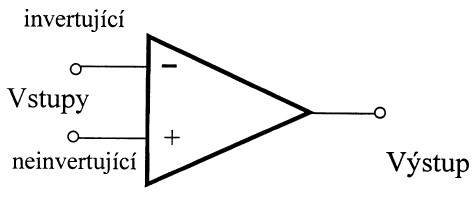
\includegraphics[scale=0.6]{scheme}
                \captionsetup{justification=centering, font=footnotesize}
                \captionof{figure}{Schematické označení operačního zesilovače.}
                \label{fig:scheme}
                \vspace{10pt}
                \raggedright   

            \subsection{Komparátor}
                Komparátor je speciální typ operačního zesilovače, který porovnává dva vstupy a generuje výstupní signál, který indikuje, který z vstupů je větší. Schema komparátoru je znázorněno na obrázku (2).
                \par Výstup komparátoru je buď v logické 1 nebo logické 0, což závisí na tom, zda je napětí na neinvertujícím vstupu vyšší než na invertujícím. 

                \vspace{10pt}   
                \par \centering
                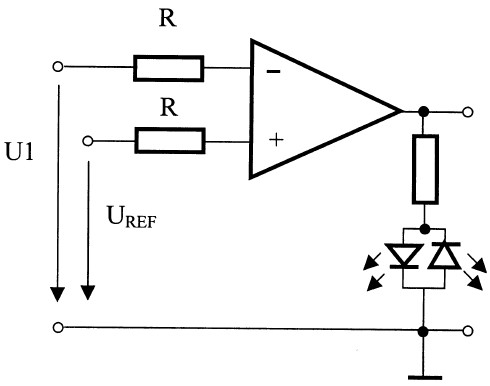
\includegraphics[scale=0.6]{komp}
                \captionsetup{justification=centering, font=footnotesize}
                \captionof{figure}{Schematické označení komparátoru.}
                \label{fig:komp}
                \vspace{10pt}
                \raggedright            
    \end{minipage}
\newpage
    \begin{minipage}[t]{0.5\textwidth} 
            \subsection{Zapojení zesilovače s invertujícím vstupem}
                Zesilovač s invertujícím vstupem je zesilovač, kde je vstupní signál přiveden na invertující vstup operačního zesilovače. Schema daného zapojení je znázorněna na obrázku (3). Výstupní signál je pak zesílený a fázově obrácený oproti vstupnímu signálu. 
                \par Vzorec pro zesílení tohoto zapojení je dán vztahem (1):
                \begin{equation}
                    U_0 = -\frac{R_2}{R_1} U_1
                \end{equation}
                kde $R_1$ a $R_2$ jsou odpory v obvodu. 
                \par Šířka pásma je maximální frekvence, při které je operační zesilovač v daném zapojení pracuje dostatečně dobře. 
                \par Tato mez se obvykle udává jako frekvence, při které zesílení klesne o 3 dB ve srovnání se ziskem nízkofrekvenčních signálů $A_{u_{max}}$ teoreticky popsaná rovnicí (1). Pokles o 3 dB odpovídá snížení zesílení na $A_{u_{max}}/\sqrt{2}$.

                \vspace{10pt}   
                \par \centering
                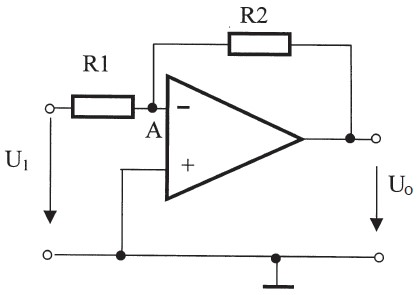
\includegraphics[scale=0.6]{inv_scheme}
                \captionsetup{justification=centering, font=footnotesize}
                \captionof{figure}{Zapojení zesilovače s invertujícím vstupem.}
                \label{fig:inv_scheme}
                \vspace{10pt}
                \raggedright  

            \subsection{Dolnofrekvenční propust}
                Dolnofrekvenční propust je obvod, který propouští signály s frekvencí nižší než je určitá mez. Schema daného zapojení je znázorněna na obrázku (4). 
                \par Vzorec pro zesílení tohoto zapojení je dán vztahem (2):
                \begin{equation}
                    A_u = -\frac{R_F}{R_A} \frac{1}{1 + i\omega C_F R_F}
                \end{equation}
                kde $R_F$ a $R_A$ jsou odpory v obvodu a $C_F$ je kapacita kondenzátoru.

            \subsection{Zapojení zesilovače s neinvertujícím vstupem}
                Zesilovač s neinvertujícím vstupem je zesilovač, kde je vstupní signál přiveden na neinvertující vstup operačního zesilovače. Schema daného zapojení je znázorněna na obrázku (5). 
    \end{minipage}
    \hspace{10pt}
    \begin{minipage}[t]{0.5\textwidth} 
                \vspace{10pt}   
                \par \centering
                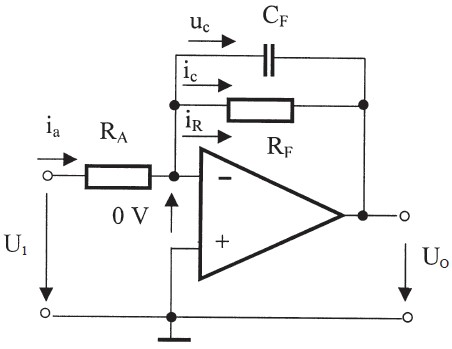
\includegraphics[scale=0.6]{low_scheme}
                \captionsetup{justification=centering, font=footnotesize}
                \captionof{figure}{Zapojení dolnofrekvenční propusti.}
                \label{fig:low_scheme}
                \vspace{10pt}
                \raggedright

                \par Vzorec pro zesílení tohoto zapojení je dán vztahem (3):
                \begin{equation}
                    U_0 = \left(1 + \frac{R_2}{R_1}\right) U_1
                \end{equation}
                kde $R_1$ a $R_2$ jsou odpory v obvodu.

                \vspace{10pt}   
                \par \centering
                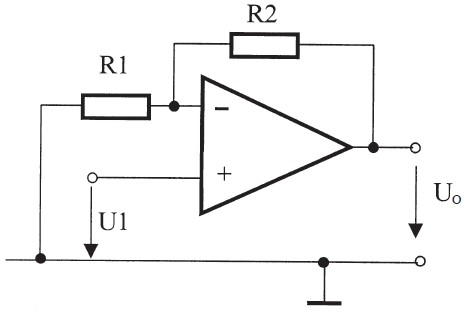
\includegraphics[scale=0.6]{non_inv_scheme}
                \captionsetup{justification=centering, font=footnotesize}
                \captionof{figure}{Zapojení zesilovače s neinvertujícím vstupem.}
                \label{fig:non_inv_scheme}
                \vspace{10pt}
                \raggedright

            \subsection{Rozdílový zesilovač}
                Rozdílový zesilovač je obvod, který zesiluje rozdíl mezi dvěma vstupy. Schema daného zapojení je znázorněna na obrázku (6). 
                \par Vzorec pro zesílení tohoto zapojení je dán vztahem (4):
                \begin{equation}
                    U_0 = U_2 \frac{R_4(R_1+R_2)}{R_1(R_3+R_4)} - U_1 \frac{R_2}{R_1} = 2(U_2 - U_1)
                \end{equation}
                kde $R_1$ a $R_2$ jsou odpory v obvodu. $R_1$ = $R_3$ = 10 $\Omega$ a $R_2$ = $R_4$ = 20 $\Omega$.

            \subsection{Derivátor}  
                Derivátor je obvod, který zpracovává vstupní signál tak, že výstupní signál je derivací vstupního signálu. Varianty derivátoru jsou znázorněny na obrázku (7).
    \end{minipage}
\newpage
    \begin{minipage}[t]{0.5\textwidth}
                \vspace{10pt}   
                \par \centering
                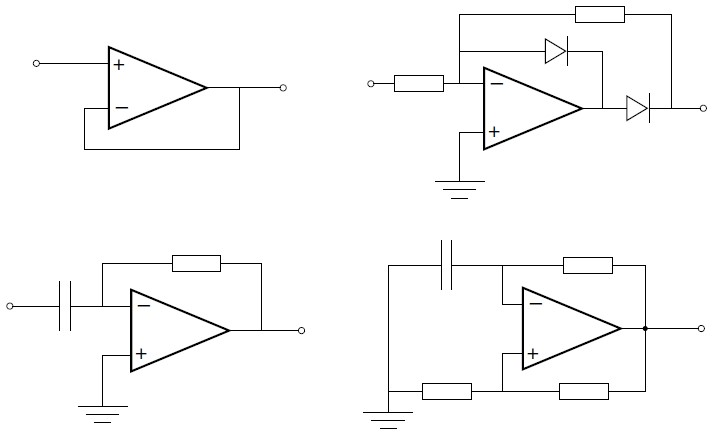
\includegraphics[scale=0.45]{deriv.jpg}
                \captionsetup{justification=centering, font=footnotesize}
                \captionof{figure}{Zapojení derivátoru.}
                \label{fig:deriv.jpg}
                \vspace{10pt}
                \raggedright

        \section{Měření}
            \subsection{Komparátor}
                Pokud je napětí na neinvertujícím vstupu vyšší než na invertujícím, jeden z diod je zapojen v opačném směru a neprotéká jím proud. Druhý diod je zapojen ve směru proudu a svítí. Když se napětí změní tak, že na invertujícím vstupu je vyšší, směr proudu v diodách se obrátí a svítí nyní druhý diod.

            \subsection{Zesilovač s invertujícím vstupem}
                Pro ověření platnosti vzorce (1) jsme změřili závislost vstupního napětí $U_0$ na výstupním napětí $U_1$. Poté jsme provedli lineární fitování, abychom určili faktor úměrnosti $\frac{R_2}{R_1}$. Výsledky jsou znázorněny v grafu (7).
                Při měření jsme použili odpory $R_1$ = 10 $\Omega$ a $R_2$ = 20 $\Omega$.  To znamená, že $\frac{R_2}{R_1}$ = -2. Z fitování byla získána následující hodnota: 
                \begin{center}
                    $\frac{R_2}{R_1}$ = -2.034 $\pm$ 0.003
                \end{center}

                \vspace{10pt}           
                \par \centering
                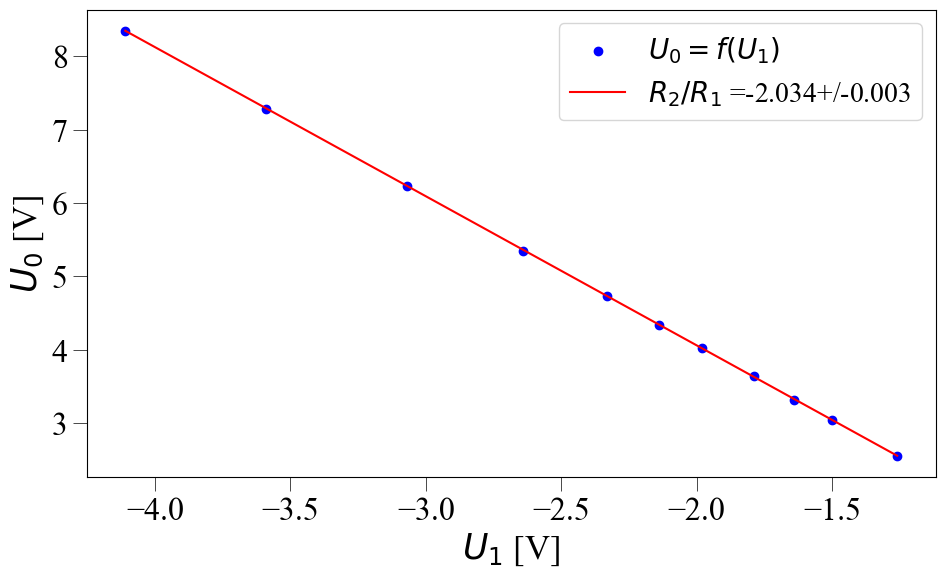
\includegraphics[scale=0.32]{inv}
                \captionsetup{justification=centering, font=footnotesize}
                \captionof{figure}{Závislost $U_0$ = $f(U_1)$ pro zesilovač s invertujícím vstupem.}
                \label{fig:inv}
                \vspace{10pt}
                \raggedright 
    \end{minipage}
    \hspace{10pt}  
    \begin{minipage}[t]{0.5\textwidth}  
                Pro určení šířky pásma jsme změřili závislost zesílení na frekvenci. Výsledky jsou znázorněny v grafu (8). Z měření jsme získali maximální hodnotu zesílení $A_{u_{max}}/\sqrt{2}$ = 3.04. Po vynesení dat do grafu (frekvenci jsme také zlogaritmovali) jsme provedli polynomickou aproximaci a poté jsme našli průsečík $A_{u_{max}}/\sqrt{2}$ na ose Y s fitovací křivkou, abychom určili optimální frekvenci $\omega$ na ose X. Získali jsme následující hodnotu $\omega$:
                \begin{center}
                    $\omega$ = 39609 Hz 
                \end{center}

                \vspace{10pt}           
                \par \centering
                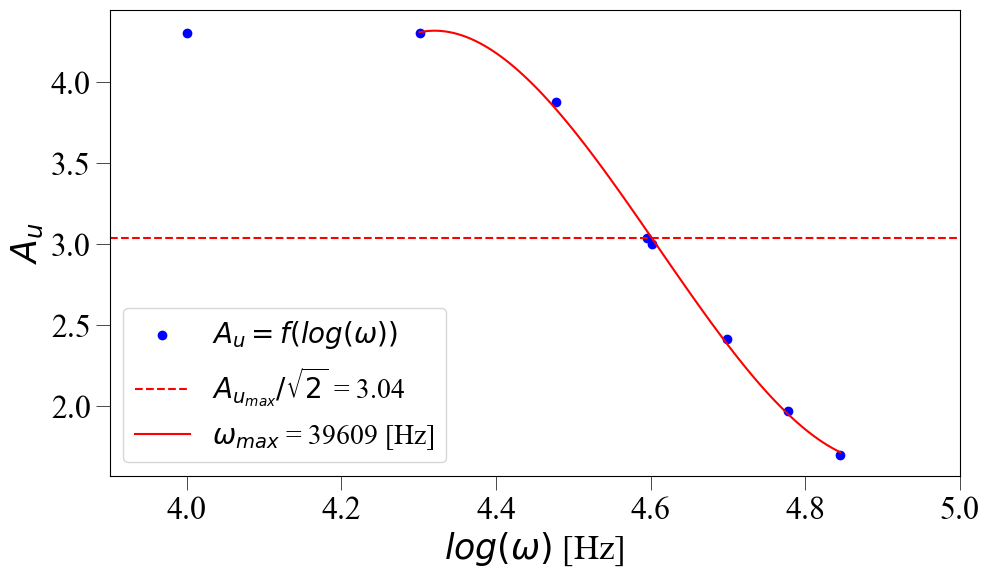
\includegraphics[scale=0.32]{inv_freq}
                \captionsetup{justification=centering, font=footnotesize}
                \captionof{figure}{Závislost $A_u$ = $f(\omega)$ pro zesilovač s invertujícím vstupem.}
                \label{fig:inv_freq}
                \vspace{10pt}
                \raggedright

            \subsection{Dolnofrekvenční propust}
                Pro určení šířky pásma dolnofrekvenční propusti jsme změřili závislost zesílení na frekvenci. Výsledky jsou znázorněny v grafu (9). Z měření jsme získali maximální hodnotu zesílení $A_{u_{max}}/\sqrt{2}$ = 7.66. Po vynesení dat do grafu (frekvenci jsme také zlogaritmovali) jsme provedli polynomickou aproximaci a poté jsme našli průsečík $A_{u_{max}}/\sqrt{2}$ na ose Y s fitovací křivkou, abychom určili optimální frekvenci $\omega$ na ose X. Získali jsme následující hodnotu $\omega$:
                \begin{center}
                    $\omega$ = 158 Hz
                \end{center}

                \vspace{10pt}           
                \par \centering
                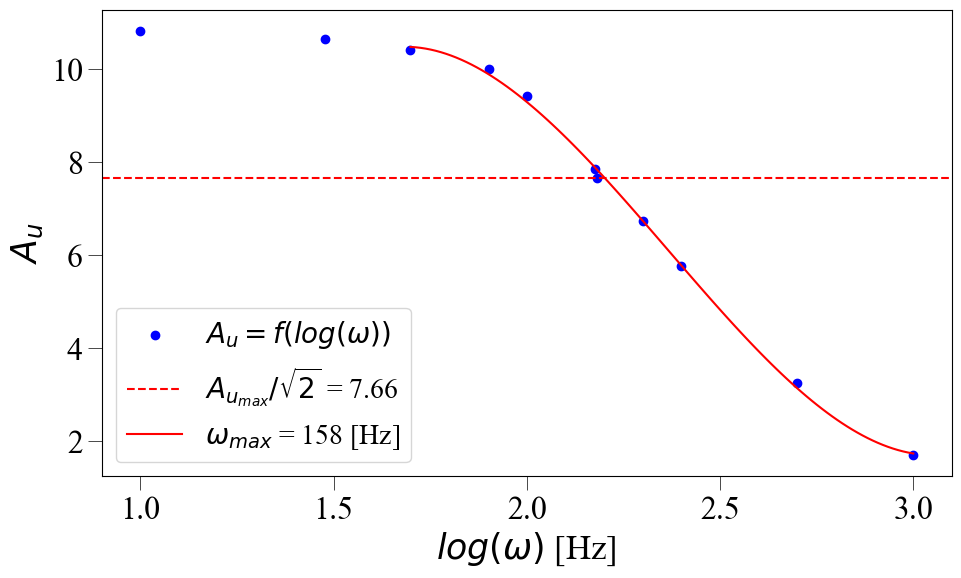
\includegraphics[scale=0.32]{low}
                \captionsetup{justification=centering, font=footnotesize}
                \captionof{figure}{Závislost $A_u$ = $f(\omega)$ pro dolnofrekvenční propust.}
                \label{fig:low}
                \vspace{10pt}
                \raggedright
    \end{minipage}
\newpage
    \begin{minipage}[t]{0.5\textwidth}
            \subsection{Zesilovač s neinvertujícím vstupem}
                Pro ověření platnosti vzorce (3) jsme změřili závislost vstupního napětí $U_0$ na výstupním napětí $U_1$. Poté jsme provedli lineární fitování, abychom určili faktor úměrnosti $\left(1 + \frac{R_2}{R_1}\right)$. Výsledky jsou znázorněny v grafu (10).
                Při měření jsme použili dvě kombinační odpory $R_{1,1}$ = 10 $\Omega$, $R_{2,1}$ = 20 $\Omega$ a $R_{1,2}$ = 20 $\Omega$, $R_{2,2}$ = 10 $\Omega$. To znamená, že $\left(1 + \frac{R_{2,1}}{R_{1,1}}\right)$ = 3 a $\left(1 + \frac{R_{2,2}}{R_{1,2}}\right)$ = 1.5. Z fitování byly získány následující hodnoty:
                \begin{center}
                    $\left(1 + \frac{R_{2,1}}{R_{1,1}}\right)$ = 2.98 $\pm$ 0.03
                    \vspace{10pt}
                    \par $\left(1 + \frac{R_{2,2}}{R_{1,2}}\right)$ = 1.500 $\pm$ 0.001
                \end{center}

                \vspace{10pt}           
                \par \centering
                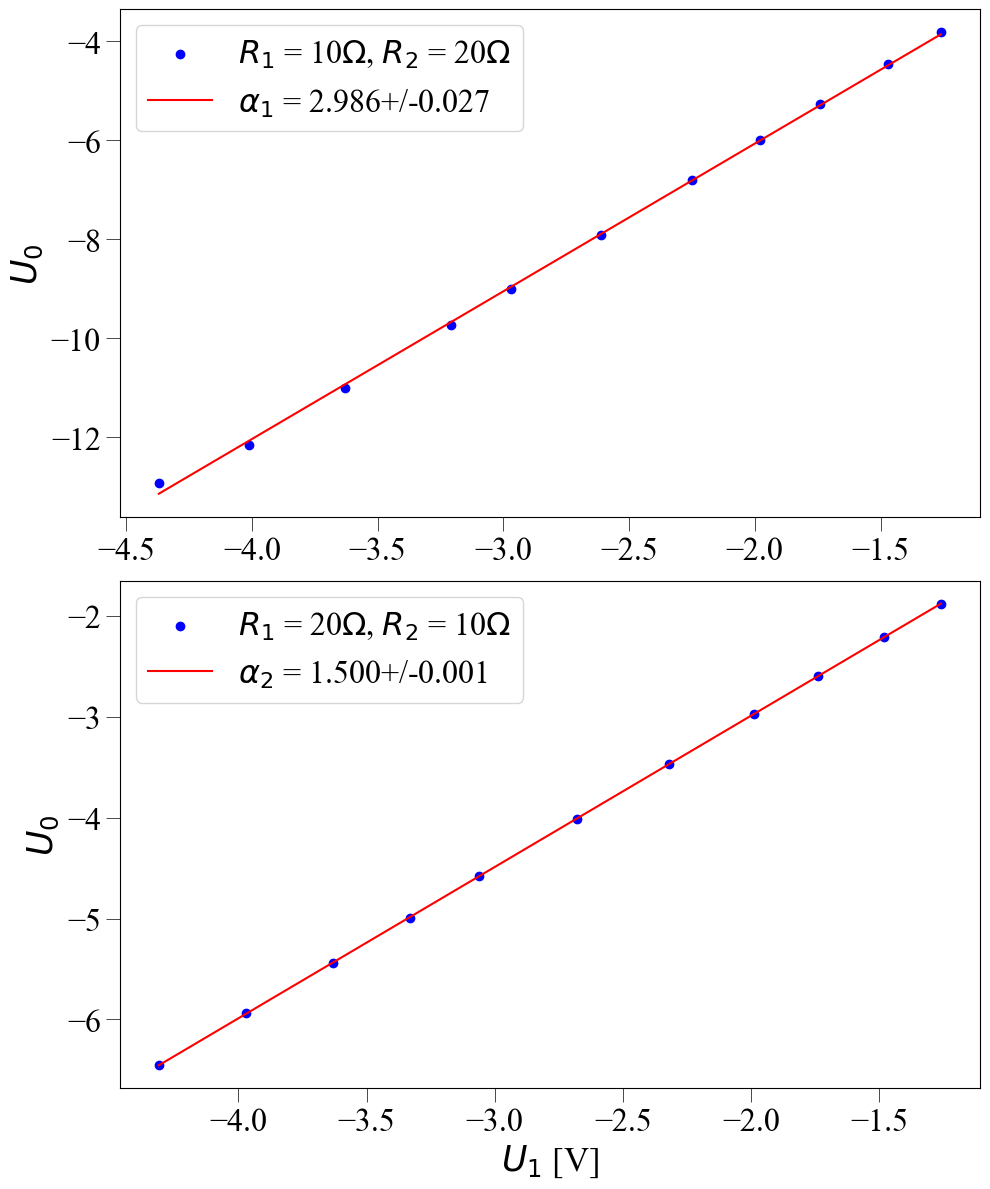
\includegraphics[scale=0.32]{non_inv}
                \captionsetup{justification=centering, font=footnotesize}
                \captionof{figure}{Závislost $U_0$ = $f(U_1)$ pro zesilovač s neinvertujícím vstupem pro dvě kombinace odporu.}
                \label{fig:non_inv}
                \vspace{10pt}
                \raggedright
            
            \subsection{Rozdílový zesilovač}
                Pro ověření platnosti vzorce (4) jsme změřili závislost vstupního napětí $U_0$ na rozdílu vstupních napětí ($U_2$-$U_1$).

    \end{minipage}
    \hspace{10pt}  
    \begin{minipage}[t]{0.5\textwidth}
                \vspace{10pt}           
                \par \centering
                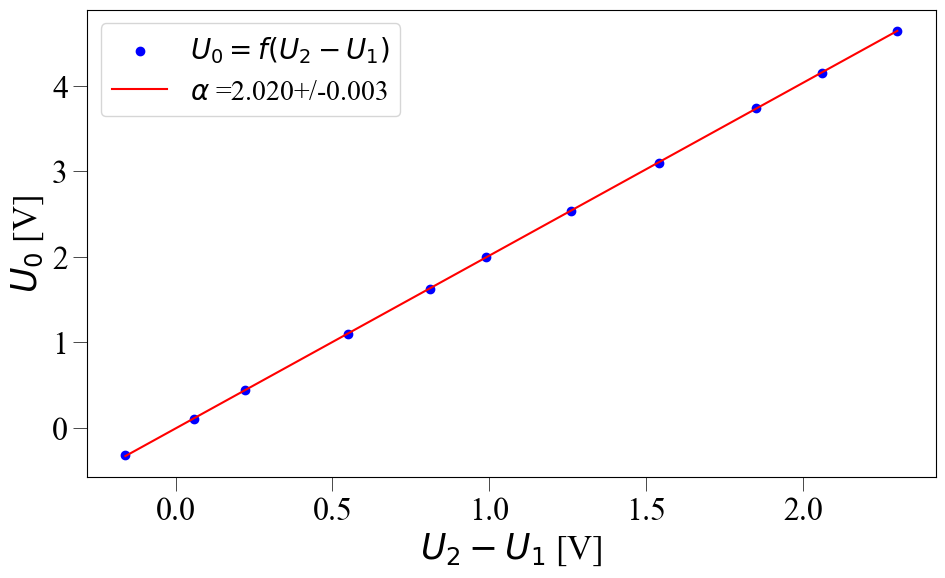
\includegraphics[scale=0.32]{diff}
                \captionsetup{justification=centering, font=footnotesize}
                \captionof{figure}{Závislost $U_0$ = $f(U_2-U_1)$ pro rozdílový zesilovač.}
                \label{fig:diff}
                \vspace{10pt}
                \raggedright

                \par Poté jsme provedli lineární fitování, abychom určili faktor úměrnosti 2. Výsledky jsou znázorněny v grafu (11). Z fitování byla získána následující hodnota:
                \begin{center}
                    $\alpha$ = 2.020 $\pm$ 0.003
                \end{center}

            \subsection{Derivační zesilovač}
                Abychom určili, který obvod zesilovače představuje derivátor, provedli jsme pozorování pomocí osciloskopu. Za tímto účelem jsme vyndali vstupní a výstupní signál, překryli je na sebe a zjistili, že když je vstupní signál sinusový, výstupní signál je kosinusový.
                \par Tím jsme zjistili, že obvod zesilovače znázorněný na obrázku (12) funguje jako derivátor.

                \vspace{10pt}           
                \par \centering
                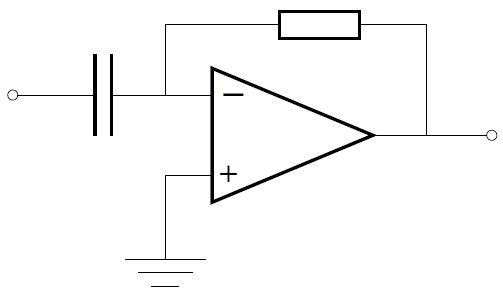
\includegraphics[scale=0.45]{derivator}
                \captionsetup{justification=centering, font=footnotesize}
                \captionof{figure}{Zapojení derivátoru.}
                \label{fig:derivator}
                \vspace{10pt}
                \raggedright

                \par Výsledky měření jsou v tabulce (1), (2), (3) a (4).
                \vspace{10pt}
                \par K výpočtu veličin a jejich nejistot byla použita knihovna Uncertinties pro Python \cite{uncertainties}. Chyby byly rozšířeny o Studentův koeficient (2-Tail Confidence Level) s ohledem na stupně volnosti pro každou hodnotu, pro interval spolehlivosti 68.27\%.
    \end{minipage}
\newpage
        \section{Závěr} 
                \par Bylo ověřeno, že komparátor reaguje na různá vstupní napětí a jejich rozdíly.
                \par Byla ověřena platnost vzorce (1) pro invertující zesilovač. Ziskaý faktor úměrnosti $\frac{R_2}{R_1}$ = -2.034 $\pm$ 0.003 byl v souladu s teoretickou hodnotou $\frac{R_2}{R_1}$ = -2. Byla určena šířka pásma daného zapojení operačního zesilovače a získána hodnota $\omega$ = 39609 Hz.
                \par Byla změřena závislost zesílení na frekvenci a z grafu této závislosti byla určena šířka pásma dolnofrekvenčního zesilovače a získána hodnota $\omega$ = 158 Hz.
                \par  Byla ověřena platnost vzorce (3) pro neinvertující zesilovač a získány faktory úměrnosti $\left(1 + \frac{R_{2,1}}{R_{1,1}}\right)$ = 2.98 $\pm$ 0.03 a $\left(1 + \frac{R_{2,2}}{R_{1,2}}\right)$ = 1.500 $\pm$ 0.001, které byly v souladu s teoretickými hodnotami $\left(1 + \frac{R_{2,1}}{R_{1,1}}\right)$ = 3 a $\left(1 + \frac{R_{2,2}}{R_{1,2}}\right)$ = 1.5.
                \par  Byla ověřena platnost vzorce (4) pro rozdílový zesilovač a získán faktor úměrnosti $\alpha$ = 2.020 $\pm$ 0.003, který byl v souladu s teoretickou hodnotou $\alpha$ = 2.
                \par Bylo zjištěno, že obvod zesilovače znázorněný na obrázku (12) plní funkci derivačního zesilovače.

                \renewcommand{\refname}{Odkazy}
                \begin{thebibliography}{9}
                    \bibitem{uncertainties}
                        Uncertainties, Dostupné online: \url{https://pypi.org/project/uncertainties}
                \end{thebibliography} 

    \begin{center}
        \section{Appendix}
            \subsection{Tabulka naměřených hodnot pro zesilovač s invertujícím vstupem}
                \pgfplotstabletypeset[
                    col sep=comma, % Defines the separator, comma for CSV
                    string type, % Treats columns as strings (not math mode)
                    every head row/.style={before row=\toprule,after row=\midrule},
                    every last row/.style={after row=\bottomrule},
                    columns/f/.style={column name=$log(\omega)$},
                    columns/U_0_A/.style={column name=A_u},
                    columns/U_0/.style={column name=U_0 [V]},
                    columns/U_1 /.style={column name=U_1 [V]},
                ]{data/inv_out.csv} 
    \end{center}
    \begin{center}
        \subsection{Tabulka naměřených hodnot pro dolnofrekvenční propust}
            \pgfplotstabletypeset[
                col sep=comma, % Defines the separator, comma for CSV
                string type, % Treats columns as strings (not math mode)
                every head row/.style={before row=\toprule,after row=\midrule},
                every last row/.style={after row=\bottomrule},
                columns/f/.style={column name=$log(\omega)$},
                columns/U_0/.style={column name=U_0 [V]},
            ]{data/low_out.csv} 
    \end{center}
\newpage    
    \begin{center}
        \subsection{Tabulka naměřených hodnot pro zesilovač s neinvertujícím vstupem}
            \pgfplotstabletypeset[
                col sep=comma, % Defines the separator, comma for CSV
                string type, % Treats columns as strings (not math mode)
                every head row/.style={before row=\toprule,after row=\midrule},
                every last row/.style={after row=\bottomrule},
                columns/U_1_1/.style={column name=U_{1,1} [V]},
                columns/U_0_1/.style={column name=U_{0,1} [V]},
                columns/U_1_2/.style={column name=U_{1,2} [V]},
                columns/U_0_2/.style={column name=U_{0,2} [V]},
            ]{data/non_inv_out.csv} 
    \end{center}
    \begin{center}
        \subsection{Tabulka naměřených hodnot pro rozdílový zesilovač}
            \pgfplotstabletypeset[
                col sep=comma, % Defines the separator, comma for CSV
                string type, % Treats columns as strings (not math mode)
                every head row/.style={before row=\toprule,after row=\midrule},
                every last row/.style={after row=\bottomrule},
                columns/U_0/.style={column name=U_0 [V]},
                columns/U_1/.style={column name=U_1 [V]},
                columns/U_2/.style={column name=U_2 [V]},
                columns/dU/.style={column name=(U_2-U_1) [V]},
            ]{data/diff_out.csv} 
    \end{center}
\end{document}